\chapter{``6D'' beam-beam interaction}

\section{Introduction} 

This chapter describes in detail the numerical method used in different codes, and in particular in SixTrack \cite{sixtracksite} and Xsuite, for the simulation of beam-beam interactions in the weak-strong framework using the ``Synchro Beam Mapping'' 
approach \cite{hirata, hirata_crossing_angle}.  This allows correctly modeling the coupling introduced by beam-beam between the longitudinal and transverse planes. The goal of this document is  in particular to provide in a compact, complete and self-consistent manner, the set of equations that are needed for the implementation in a numerical code. 
Complementary information can be found in \cite{bb6dslides}, including graphical representations of the procedure presented in this note and several validation tests.

The effect of a ``crossing angle'' in an arbitrary ``crossing plane'' with respect to the assigned reference frame is taken into account with a suitable coordinate transformation following the approach described in \cite{hirata, beam_beam}. The employed description of the strong beam allows the correct inclusion of the hour-glass effect as well as the linear coupling at the interaction point, following the treatment presented in \cite{beam_beam}. 


If not differently stated in an explicit way in the following, all coordinates are given in the reference system defined by the closed orbit of the weak beam, which is traveling with positive speed along the $s$ direction. The Interaction Point (IP) is located at $s$=0 and the crossing plane is defined by as the angle that the strong beam forms with the $s$-axis. In the presence of an offset between the beams (separation), the orientation of the reference system is defined by the closed orbit of the weak beam and the system is centered at the IP location as defined for the strong beam. Therefore the strong beam passes always through the origin of the reference frame.




\section{Direct Lorentz boost (for the weak beam)}
\label{sec:directboost}

We want to transform the coordinates by moving to a Lorentz boosted frame in which the collision is head-on (i.e. $p_x=p_y=0$ for the strong beam and for the reference particle of the weak beam). We call $\phi$ the half crossing angle and $\alpha$ the angle that the crossing plane makes with respect to the $x-z$ plane. For this purpose, we perform a transformation which actually includes four operations (more details can be found in Appendix~\ref{app:boost} and in~\cite{bb6dslides, beam_beam}):
\begin{itemize}
\item Transform the accelerator positions and momenta into Cartesian coordinates (which can then be Lorentz boosted);
\item Rotate particle coordinates to the ``barycentric'' reference frame;
\item Perform the Lorentz boost;
\item Drift all the particles back to $s=0$ (as not all particles with $s=0$ are fixed points of the transformation, and we are tracking with respect to $s$ and not with respect to time).
\end{itemize}

We name the original accelerator coordinates (as defined in the SixTrack Physics Manual \cite{sixtracksite}):
\begin{equation}
\left(x, p_x, y, p_y, \sigma, \delta\right)
\end{equation}
and the transformed coordinates:
\begin{equation}
\left(x^*, p_x^*, y^*, p_y^*, \sigma^*, \delta^*\right)
\end{equation}

%\textit{Note that in \cite{refpaper} $z$ is actually $\sigma$ and $p_z$ is actually $\delta$!}


We start by computing the drift Hamiltonian in the original coordinates (we are doing a Lorentz transformation, therefore constants matter as we are assuming that $h$ is the total energy of the particle):
\begin{equation}
h = \delta + 1 -\sqrt{\left(1+\delta\right)^2-p_x^2-p_y^2}
\end{equation}

We transform the momenta:
\begin{align}
p_x^* &= \frac{p_x}{\cos \phi} - h \cos \alpha \frac{\tan \phi}{\cos \phi} \label{eq:px}\\ 
p_y^* & = \frac{p_y}{\cos \phi} - h \sin \alpha \frac{\tan \phi}{\cos \phi}\\ 
\delta^* & = \delta -p_x \cos \alpha \tan \phi - p_y \sin \alpha \tan \phi +h \tan^2 \phi \label{eq:delta}
\end{align}

In order to calculate the angles in the transformed frame, we evaluate:
\begin{equation}
p^*_z  =  \sqrt{\left(1+\delta^*\right)^2-{p_x^*}^2-{p_y^*}^2}
\end{equation}

We can now evaluate the following derivatives of the transformed Hamiltonian (from Hamilton's equations it can be easily seen that these are the angles in the boosted frame):

\begin{align}
h^*_x &= \frac{\partial h^*}{\partial p^*_x} = \frac{p^*_x}{p^*_z}\\
h^*_y &= \frac{\partial h^*}{\partial p^*_y} = \frac{p^*_y}{p^*_z}\\
h^*_\sigma &= \frac{\partial h^*}{\partial \delta} = 1-\frac{\delta^*+1}{p^*_z}
\end{align}

These can be used to build the following matrix:

\begin{equation}
L  =\left( \begin{matrix}

\left( 1 + h^*_x \cos \alpha \sin \phi\right) & h^*_x \sin \alpha \sin \phi & \cos \alpha \tan \phi \\
h_y^* \cos \alpha \sin \phi & \left( 1 + h^*_y \sin \alpha \sin \phi\right) & \sin \alpha \tan \phi\\
h_\sigma^* \cos \alpha \sin \phi & h_\sigma^* \sin \alpha \sin \phi  & \frac{1}{\cos \phi}\\
\end{matrix} \right)
\label{eq:Lmat}
\end{equation}

which can then be used to transform the test-particle positions:

\begin{equation}
\left( \begin{matrix}
x^*\\
y^*\\
\sigma^*
\end{matrix}\right) = 
L 
\left( \begin{matrix}
x\\
y\\
\sigma
\end{matrix}\right)
\end{equation}


\section{Syncrho-beam mapping}

Following the approach introduced in~\cite{hirata}, the strong beam is sliced along z. A common approach is to use constant-charge slices (see Appendix~\ref{app:slicing}). For each particle in the weak beam and for each slice in the strong beam we perform the following.
~\\

We identify the position of the Collision Point (CP):

\begin{equation}
S = \frac{\sigma^*-\sigma^*_\textrm{sl}}{2}
\label{eq:sdef}
\end{equation}

Here $\sigma^*$ is defined in the reference system of the weak beam ( $\sigma^*>0$ for particles at the head of the weak bunch) while $\sigma^*_\textrm{sl}$ is defined in the reference system of the strong beam ( $\sigma^*_\textrm{sl}>0$ for particles at the head of the strong bunch). $S$ is the coordinate of the collision point \underline{in the reference system of the weak beam} (from Eq.~\ref{eq:sdef}, we can see that particles at the head of the weak bunch, collide with particles at the tail of the strong bunch at $S>0$). 
~\\

\textit{N.B. Here we are making an approximation since we are assuming that particles are moving at the speed of light along z independently on their angles. This means that the presented approach works only for small particle angles. It is for this reason that we need to Lorentz boost to get rid of the crossing angle and we cannot just move to the reference of the strong beam using a rotation (in this case the weak beam would have large angles).}
~\\

We now evaluate the transverse position of the particle at the CP, with respect to the centroid of the slice, taking into account the particle angles :
\begin{align}
\overline{x}^* &= x^* + p^*_x S - (x^*_\textrm{sl} - p^*_{x, \textrm{sl}} S)\\
\overline{y}^* &= y^* + p^*_y S - (y^*_\textrm{sl} - p^*_{y, \textrm{sl}} S)
\end{align}
Here $x^*_\textrm{sl}$, $y^*_\textrm{sl}$, $p^*_{x, \textrm{sl}}$ and $p^*_{y, \textrm{sl}}$  are defined \underline{in the coordinate system of the weak beam}. The momenta of the strong slice appear with a negative sign since in the weak frame the strong slice is travelling "backwards".
~\\

\subsection{Propagation of the strong beam to the collision point}

The distribution of the strong beam in the transverse phase-space can be written using the $\Sigma$-matrix~\cite{wolski2014beam}:
\begin{equation}
f(\eta) = f_0 e^{{-\eta}^{\mathrm{T}} \Sigma^{-1}\eta}
\end{equation}

where:
\begin{equation}
\eta = \left(
\begin{matrix}
x\\
p_x\\
y\\
p_y
\end{matrix}
\right)
\end{equation}

Points having same phase space density lie on hyper-elliptic manifolds defined by the equation:
\begin{equation}
\eta^\mathrm{T}\Sigma^{-1}\eta = \mathrm{const.}
\label{eqellipse}
\end{equation}

Further considerations on the $\Sigma$-matrix can be found in Appendix~\ref{app:sigma}.

We transform the $\Sigma$-matrix at the Interaction Point to take into account the Lorentz Boost:
\begin{align}
\Sigma^{*0}_{11} &= \Sigma_{11} ^0\\
\Sigma^{*0}_{12} &= \Sigma_{12} ^0/\cos \phi\\
\Sigma^{*0}_{13} &= \Sigma_{13} ^0\\
\Sigma^{*0}_{14} &= \Sigma_{14} ^0/\cos \phi\\
\Sigma^{*0}_{22} &= \Sigma_{22} ^0/\cos^2 \phi\\
\Sigma^{*0}_{23} &= \Sigma_{23} ^0/\cos \phi\\
\Sigma^{*0}_{24} &= \Sigma_{24} ^0/\cos^2 \phi\\
\Sigma^{*0}_{33} &= \Sigma_{33} ^0\\
\Sigma^{*0}_{34} &= \Sigma_{34} ^0/\cos \phi\\
\Sigma^{*0}_{44} &= \Sigma_{44} ^0/\cos^2 \phi\\
\end{align}

We transport the position part of the boosted $\Sigma$-matrix to the CP (here we are taking into account hourglass effect, assuming that we are in a drift space):
\begin{align}
\Sigma^*_{11} &= \Sigma_{11} ^{*0}+2 \Sigma_{12} ^{*0} S+\Sigma_{22} ^{*0} S^2 \label{eq:TranspSig11}\\
\Sigma^*_{33} &= \Sigma_{33} ^{*0}+2 \Sigma_{34} ^{*0} S +\Sigma_{44} ^{*0} S^2\label{eq:TranspSig33}\\
\Sigma^*_{13} &= \Sigma_{13} ^{*0}+\left(\Sigma_{14} ^{*0} +\Sigma_{23}^{*0}\right) S +\Sigma_{24} ^{*0} S^2\label{eq:TranspSig13}
\end{align}

The $\Sigma$-matrix is given \underline{in the reference system of the weak beam}.% which is not what  \cite{refpaper} is doing.
~\\
For singular cases we will also need to transport the other terms:
\begin{align}
\Sigma^*_{12} &= \Sigma_{12} ^{*0}+\Sigma_{22} ^{*0}S\\
\Sigma^*_{14} &= \Sigma_{14} ^{*0}+\Sigma_{24} ^{*0}S\\
\Sigma^*_{22} &= \Sigma_{22} ^{*0}\\
\Sigma^*_{23} &= \Sigma_{23} ^{*0}+\Sigma_{24} ^{*0}S\\
\Sigma^*_{24} &= \Sigma_{24} ^{*0}\\
\Sigma^*_{34} &= \Sigma_{34} ^{*0}+\Sigma_{44} ^{*0}S\\
\Sigma^*_{44} &= \Sigma_{44} ^{*0}
\end{align}



We introduce the following three auxiliary quantities:
\begin{align}
R\left(S \right)  &= \Sigma^*_{11} - \Sigma^*_{33}\\
W\left(S\right) &= \Sigma^*_{11} + \Sigma^*_{33}\\
T\left( S \right) &= {R^2 + 4 {\Sigma^*_{13}}^2 } \label{eq:Tfun}
\end{align}

The following derivatives will be needed in the following:
\begin{align}
\frac{\partial R}{\partial S}  &= 2\left(\Sigma_{12} ^0 - \Sigma_{34}^0\right) + 2S\left(\Sigma_{22} ^0 - \Sigma_{44}^0\right) \\ 
\frac{\partial W}{\partial S} &= 2\left(\Sigma_{12} ^0 + \Sigma_{34}^0\right) + 2S\left(\Sigma_{22} ^0 + \Sigma_{44}^0\right) \\
\frac{\partial \Sigma^*_{13}}{\partial S}  &= \Sigma_{14} ^0 + \Sigma_{23} ^0 + 2\Sigma_{24} ^0 S\\
\frac{\partial T}{\partial S}  &= 2R \frac{\partial R}{\partial  S} +8  \Sigma^*_{13} \frac{\partial \Sigma^*_{13}}{\partial  S}
\end{align}

We will now compute, at the location of the CP, the coupling angle $\theta$, defining a reference frame in which the beam is decoupled.
We will call $\hat{x}$ and $\hat{y}$ the coordinates in the decoupled frame and  $\hat{\Sigma}^*_{11}$,  $\hat{\Sigma}^*_{33}$ the corresponding squared beam sizes. The angle $\theta$ is defined as the angle between the $\hat{x}$-axis and the $x$-axis.

These quantities can be found by diagonalizing the $x-y$ block of the $\Sigma$-matrix.
We will make determination choices (Eqs.~\ref{eq:cos2theta}, \ref{eq:sincostheta} and \ref{eq:sigmashat}) so that the set $(\theta, \hat{\Sigma}^*_{11}, \hat{\Sigma}^*_{33})$ is uniquely defined and the coupling angle $\theta$ lies in the interval:
\begin{align}
-\frac{\pi}{4}<\theta<\frac{\pi}{4}
\end{align}

Different cases need to be treated separately:
~\\

\textbf{\underline{Case T>0, $\left|\Sigma^*_{13}\right|$>0}}
~\\

We evaluate the coupling angle at the position of the CP in the boosted frame:
\begin{equation}
\cos 2\theta = \textrm{sgn} \left(\Sigma^*_{11} - \Sigma^*_{33}\right)\frac{\Sigma^*_{11} - \Sigma^*_{33}}{\sqrt{\left(\Sigma^*_{11} - \Sigma^*_{33}\right)^2 + 4 {\Sigma^*_{13}}^2 }}
\end{equation}

Or more synthetically:
\begin{equation}
\cos 2\theta = \textrm{sgn}(R)\frac{R}{\sqrt{T}}
\label{eq:cos2theta}
\end{equation}

In the following we will need also the derivative of this quantity:
\begin{equation}
\frac{\partial }{\partial S} \left[ \cos 2\theta \right] =  \textrm{sgn}(R)
\left(\frac{\partial R}{\partial S} \frac{1}{\sqrt{T}}-\frac{R}{2\left( \sqrt{T}\right)^3}\frac{\partial T}{\partial S}\right)
\end{equation}

It can be proved that \cite{beam_beam}:
\begin{align}
\cos \theta &= \sqrt{\frac{1}{2}\left(1 + \cos 2\theta \right)}\\
\sin \theta &= \textrm{sgn}(R)\textrm{sgn}(\Sigma^*_{13}) \sqrt{\frac{1}{2}\left(1 - \cos 2\theta \right)}
\label{eq:sincostheta}
\end{align}
%Here $\theta$ is defined \underline{in the reference system of the weak beam}. For this reason $\sin \theta$ has opposite sign with respect to \cite{refpaper}. 

%\textit{N.B. It seems that in sixtrack the term $\Sigma^*_{13}$ in the sgn is not there. Can this compensate for the different convention above? To be investigated...}
~\\

The corresponding derivatives are given by (see Eq. 2.64 in \cite{refpaper}):
\begin{align}
\frac{\partial }{\partial S} \cos \theta =& \frac{1}{4 \cos \theta} \frac{\partial }{\partial S} \cos 2\theta \\
\frac{\partial }{\partial S} \sin \theta =& -\frac{1}{4 \sin \theta} \frac{\partial }{\partial S} \cos 2\theta \label{eq:dS_sintheta}
\end{align}

The squared beam sizes in the rotated (un-coupled) boosted frame are given by:

\begin{align}
\hat{\Sigma}^*_{11} &= \frac{1}{2}\left[ \left(\Sigma^*_{11} + \Sigma^*_{33}\right) +\textrm{sgn}\left(\Sigma^*_{11} - \Sigma^*_{33}\right)\sqrt{\left(\Sigma^*_{11} - \Sigma^*_{33}\right)^2 + 4 {\Sigma^*_{13}}^2 }\right] \\
\hat{\Sigma}^*_{33} &= \frac{1}{2}\left[ \left(\Sigma^*_{11} + \Sigma^*_{33}\right) -\textrm{sgn}\left(\Sigma^*_{11} - \Sigma^*_{33}\right)\sqrt{\left(\Sigma^*_{11} - \Sigma^*_{33}\right)^2 + 4 {\Sigma^*_{13}}^2 }\right] 
\label{eq:sigmashat}
\end{align}


Equation~\ref{eq:sigmashat} can be written in a compact form as:

\begin{align}
\hat{\Sigma}^*_{11} &= \frac{1}{2}\left(W + \textrm{sgn}(R)\sqrt{T} \right)\\
\hat{\Sigma}^*_{33} &= \frac{1}{2}\left(W - \textrm{sgn}(R)\sqrt{T} \right) \label{eq:Sigmashat}
\end{align}




The corresponding derivatives, which will be needed in the following, are given by:
\begin{align}
\frac{\partial }{\partial S} \left[\hat{\Sigma}^*_{11} \right] = \frac{1}{2}\left(\frac{\partial W}{\partial S} + \textrm{sgn}(R)\frac{1}{2\sqrt{T}}\frac{\partial T}{\partial S}  \right)\\
\frac{\partial }{\partial S} \left[\hat{\Sigma}^*_{33} \right] = \frac{1}{2}\left(\frac{\partial W}{\partial S} - \textrm{sgn}(R)\frac{1}{2\sqrt{T}}\frac{\partial T}{\partial S}  \right)\label{eq:dS_Sigmas}
\end{align}

\textbf{\underline{Case T>0, $\left|\Sigma^*_{13}\right|$=0:}}
~\\

The treatment of the previous case is still applicable with the exception of Eq.~\ref{eq:dS_sintheta} in which the denominator becomes zero.
This happens when $\Sigma^*_{13}$=0, which implies $\sqrt{T}=\left| R \right|$ and therefore $\cos 2 \theta = 1$. The case $T=0$ will be treated separately later, therefore here we can assume $\left| R \right|>0$. We can expand with respect to ${\Sigma^*_{13}}/{R}$ obtaining:

\begin{equation}
\cos 2 \theta = \frac{\left| R \right|}{\sqrt{R^2+4 {\Sigma^*_{13}}^2}} = \frac{1}{\sqrt{1+4 \frac{{\Sigma^*_{13}}^2}{R^2}}} \simeq \frac{1}{1+2 \frac{{\Sigma^*_{13}}^2}{R^2}} \simeq 1-2 \frac{{\Sigma^*_{13}}^2}{R^2}
\end{equation}

Replacing these result in Eq.~\ref{eq:sincostheta} we obtain:

\begin{equation}
\sin \theta = \mathrm{sgn}(R)\mathrm{sgn}(\Sigma^*_{13})\frac{\left| \Sigma^*_{13} \right|}{\left| R \right|} = \frac{\Sigma^*_{13} }{ R } \label{eq:spacialsintheta}
\end{equation}





We call $S_0$ the location at which ${\Sigma}^*_{13}=0$. At this location we define the auxiliary quantities:
\begin{align}
c =& \Sigma^*_{14} + \Sigma^*_{23}\\
d =& \Sigma^*_{24}
\end{align}

We introduce $\Delta S = S - S_0$ and we can write using Eqs.~\ref{eq:TranspSig11}--\ref{eq:TranspSig13}:
\begin{equation}
\Sigma^*_{13} = c \Delta S +d \Delta S^2 \label{eq:sig13spec}
\end{equation}

By taking the derivative of Eq.~\ref{eq:spacialsintheta} and using Eq.~\ref{eq:sig13spec} we obtain:
\begin{equation}
\frac{\partial }{\partial S} \sin \theta =\frac{1}{R^2}\left[\left(c + 2d \Delta S \right) R \ - \frac{\partial R }{\partial S}\left(c\Delta S + d \Delta S^2 \right)\right]
\end{equation}

In the implementation we need only the value for $\Delta S$=0, which is simply given by:
\begin{equation}
\frac{\partial }{\partial S} \sin \theta =\frac{c}{R}
\end{equation}
 
 
 
\textbf{\underline{Case T=0, $\left| c \right|$>0}}
~\\

Special care has to be taken at sections $S_0$ at which ${\Sigma}^*_{11}={\Sigma}^*_{33}$ and ${\Sigma}^*_{13}=0$ as Eqs.~\ref{eq:cos2theta}  and \ref{eq:dS_Sigmas} cannot be evaluated directly. Also in this case we define:
\begin{equation}
\Delta S = S - S_0
\end{equation}

At the location of the apparent singularity ($\Delta S$=0) we define the auxiliary quantities:
\begin{align}
a =& \Sigma^*_{12} - \Sigma^*_{34}\\
b =& \Sigma^*_{22} - \Sigma^*_{44}\\
c =& \Sigma^*_{14} + \Sigma^*_{23}\\
d =& \Sigma^*_{24} 
\end{align}

and therefore, using Eqs.~\ref{eq:TranspSig11}--\ref{eq:TranspSig13}, we can write:
\begin{align}
&R = 2a \Delta S + b \Delta S^2 \label{eq:specR}\\
&\Sigma^*_{13} =c \Delta S +d \Delta S^2\label{eq:specS13}
\end{align}

With these definitions the function $T$ (defined by Eq.~\ref{eq:Tfun}) can be expanded around $\Delta S =0$ (using the Eqs.~\ref{eq:TranspSig11}, \ref{eq:TranspSig33}, \ref{eq:TranspSig13}):
\begin{equation}
T = \Delta S^2\left[\left(2a +b \Delta S \right)^2 +4\left( c +d \Delta S\right)^2\right]
\label{eq:Tapprox}
\end{equation}

Replacing Eq.~\ref{eq:Tapprox} in Eq.~\ref{eq:cos2theta} allows  removing the apparent singularity:
\begin{equation}
\cos 2 \theta = \frac{\left| 2a+b \Delta S\right|}{\sqrt{\left(2a +b \Delta S \right)^2 +4\left( c +d \Delta S\right)^2}}
\label{eq:cost_spc}
\end{equation}

This can be derived obtaining:
\begin{align}
\frac{\partial }{\partial S} \left[ \cos 2\theta \right] &= \mathrm{sgn}(2a+b \Delta S)\left[
\frac{b}{\sqrt{\left(2a +b \Delta S \right)^2 +4\left( c +d \Delta S\right)^2}}
\right. \nonumber \\  &\left. \qquad \qquad \qquad \qquad \qquad
-\frac{(2a+b\Delta S)(2ab+b^2 \Delta s +4 c d+ 4 d^2 \Delta S)}{\left(\sqrt{\left(2a +b \Delta S \right)^2 +4\left( c +d \Delta S\right)^2}\right)^3}
\right]
\end{align}

Similarly, replacing Eq.~\ref{eq:Tapprox} in Eq.~\ref{eq:Sigmashat} we obtain:
\begin{align}
\hat{\Sigma}^*_{11} &= \frac{W}{2} + \frac{1}{2} \mathrm{sgn}\left(2a\Delta S + b \Delta S^2\right)\left| \Delta S\right| \sqrt{\left(2a +b \Delta S \right)^2 +4\left( c +d \Delta S\right)^2}\\
\hat{\Sigma}^*_{33} &= \frac{W}{2} - \frac{1}{2} \mathrm{sgn}\left(2a\Delta S + b \Delta S^2\right)\left| \Delta S\right| \sqrt{\left(2a +b \Delta S \right)^2 +4\left( c +d \Delta S\right)^2}\label{eq:SigmasSing}
\end{align}

This can be derived obtaining:
\begin{align}
\frac{\partial }{\partial S} \left[\hat{\Sigma}^*_{11} \right] =& \frac{1}{2}\frac{\partial W }{\partial S}
+\frac{1}{2}\mathrm{sgn}\left(2a\Delta S +b \Delta S^2 \right)\mathrm{sgn}(\Delta S)\left[
\sqrt{\left(2a +b \Delta S \right)^2 +4\left( c +d \Delta S\right)^2}
\right. \nonumber \\ & \qquad  \qquad \qquad \qquad \qquad  \qquad \qquad\left. 
+\frac{\Delta S \left(2ab+b^2 \Delta s +4 c d+ 4 d^2 \Delta S \right)}{\sqrt{\left(2a +b \Delta S \right)^2 +4\left( c +d \Delta S\right)^2}}
\right] \\
\frac{\partial }{\partial S} \left[\hat{\Sigma}^*_{33} \right] =& \frac{1}{2}\frac{\partial W }{\partial S}
-\frac{1}{2}\mathrm{sgn}\left(2a\Delta S +b \Delta S^2 \right)\mathrm{sgn}(\Delta S)\left[
\sqrt{\left(2a +b \Delta S \right)^2 +4\left( c +d \Delta S\right)^2}
\right. \nonumber \\ & \qquad  \qquad \qquad \qquad \qquad  \qquad \qquad\left. 
+\frac{\Delta S \left(2ab+b^2 \Delta s +4 c d+ 4 d^2 \Delta S \right)}{\sqrt{\left(2a +b \Delta S \right)^2 +4\left( c +d \Delta S\right)^2}}
\right] 
\end{align}

In the implementation only the values at $\Delta S$=0 are needed. For this case the obtained results above can be simplified as:
\begin{equation}
\cos 2 \theta = \frac{\left| 2a\right|}{2\sqrt{a^2 + c^2}}
\end{equation}

\begin{equation}
\frac{\partial }{\partial S} \left[ \cos 2\theta \right] = \mathrm{sgn}(2a)\left[
\frac{b}{2\sqrt{a^2 + c^2 }}-\frac{a(ab+2cd)}{2\left(\sqrt{a^2 + c^2}\right)^3}
\right]
\end{equation}

\begin{align}
\hat{\Sigma}^*_{11} &= \frac{W}{2}\\
\hat{\Sigma}^*_{33} &= \frac{W}{2}
\end{align}

\begin{align}
\frac{\partial }{\partial S} \left[\hat{\Sigma}^*_{11} \right] =& \frac{1}{2}\frac{\partial W }{\partial S}
+ \mathrm{sgn}(2a)\sqrt{a^2 + c^2 }
\\
\frac{\partial }{\partial S} \left[\hat{\Sigma}^*_{33} \right] =&\frac{1}{2}\frac{\partial W }{\partial S}
- \mathrm{sgn}(2a)\sqrt{a^2 + c^2 }
\end{align}

Eqs.~\ref{eq:sincostheta} and~\ref{eq:dS_sintheta} can still be used to evaluate $\sin \theta$ and $\cos \theta$ and the corresponding derivatives, once we assume that $\mathrm{sgn}(0) = 1$ and noticing from Eqs.~\ref{eq:specR} and \ref{eq:specS13} that for small $\Delta S$:
\begin{equation}
\mathrm{sgn}(R)\mathrm{sgn}(\Sigma^*_{13}) = \mathrm{sgn}(a)\mathrm{sgn}(c)
\end{equation}


\textbf{\underline{Case T=0, c=0, $\left| a \right|$>0}}
~\\

The treatment of the previous case is still applicable with the exception of Eq.~\ref{eq:dS_sintheta} in which the denominator becomes zero.

For this case we can write (from Eq.~\ref{eq:cost_spc}) around the point where this condition is verified:
\begin{equation}
\cos 2\theta =  \frac{1}{\sqrt{1+\frac{4d^2 \Delta S^2}{\left(2a +b \Delta S\right)^2}}} \simeq  
1-\frac{2d^2 \Delta S^2}{\left(2a +b \Delta S\right)^2}
\label{eq:cos2theta_manip}
\end{equation}

We notice from Eqs.~\ref{eq:specR} and \ref{eq:specS13} that for small $\Delta S$:
\begin{equation}
\mathrm{sgn}(R)\mathrm{sgn}(\Sigma^*_{13}) = \mathrm{sgn}(a)\mathrm{sgn}(d)\mathrm{sgn}(\Delta S)\label{eq:signsin_sing}
\end{equation}

Replacing Eq.~\ref{eq:cos2theta_manip} and \ref{eq:signsin_sing} into in Eq.~\ref{eq:sincostheta}
we obtain:
\begin{equation}
\sin\theta =  \frac{d\Delta S}{2a} \left| 1 - \frac{b \Delta S}{2a}\right|
\end{equation}

which can be derived in $\Delta S = 0$ obtaining:
\begin{equation}
\frac{\partial }{\partial S} \sin \theta =\frac{d}{2a} 
\end{equation}

The case in which also $d=0$ is (or is equivalent to) the uncoupled case as $\Sigma^*_{13}$ is zero for all $S$.
~\\


\textbf{\underline{Case T=0, c=0, a=0}}
~\\

Around the apparently singular point we can write:
\begin{align}
&R = b \Delta S^2\\
&\Sigma^*_{13} =d \Delta S^2
\end{align}

Therefore:
\begin{equation}
T = S^4\left( b^2 + 4 d^2\right)
\end{equation}

and:
\begin{equation}
\cos 2 \theta = \frac{\left|b\right|}{\sqrt{b^2+4d^2}}
\end{equation}

which is a constant. Eqs. \ref{eq:sincostheta} and \ref{eq:dS_sintheta} can still be used to evaluate $\sin \theta$ and $\cos \theta$ while the corresponding derivatives vanish:

This can be derived obtaining:
\begin{align}
\frac{\partial }{\partial S} \cos \theta &= 0\\
\frac{\partial }{\partial S} \sin \theta &= 0
\end{align}

Replacing $a=c=0$ into Eq \ref{eq:SigmasSing} we obtain:
\begin{align}
\hat{\Sigma}^*_{11}  =& \frac{W}{2}
+\frac{1}{2}\mathrm{sgn}(b)\Delta S^2\sqrt{b^2+4d^2} \\
\hat{\Sigma}^*_{33} =& \frac{W}{2}
-\frac{1}{2}\mathrm{sgn}(b)\Delta S^2\sqrt{b^2+4d^2}
\end{align}

and:

\begin{align}
\frac{\partial }{\partial S} \left[\hat{\Sigma}^*_{11} \right] =& \frac{1}{2}\frac{\partial W }{\partial S}\\
\frac{\partial }{\partial S} \left[\hat{\Sigma}^*_{33} \right] =& \frac{1}{2}\frac{\partial W }{\partial S}
\end{align}

The case in which also $d=0$ is (or is equivalent to the uncoupled case) as $\Sigma^*_{13}$ is zero for all $S$.




\subsection{Forces and kicks on weak beam particles}

The positions of the weak beam particle in the un-coupled boosted frame are given by:
\begin{align}
\hat{\overline{x}}^* &= \overline{x}^*\cos \theta  + \overline{y}^*\sin \theta \\
\hat{\overline{y}}^* &= -\overline{x}^*\sin \theta  + \overline{y}^* \cos \theta
\end{align}

In the following we will also need to evaluate:
\begin{align}
\frac{\partial }{\partial S} \left[\hat{\overline{x}}^*\left(\theta (S)\right) \right] &= 
 \frac{\partial \overline{x}^* }{\partial S}  \cos \theta
+ \overline{x}^*  \frac{\partial }{\partial S} \left[ \cos \theta \right] 
+ \frac{\partial \overline{y}^* }{\partial S}  \sin \theta
+ \overline{y}^*\frac{\partial }{\partial S} \left[ \sin \theta \right]  \\
\frac{\partial }{\partial S} \left[\hat{\overline{y}}^*\left(\theta (S)\right) \right] &= 
- \frac{\partial \overline{x}^* }{\partial S}  \sin \theta
-\overline{x}^*  \frac{\partial }{\partial S} \left[ \sin \theta \right] 
+  \frac{\partial \overline{y}^* }{\partial S}  \cos \theta
+ \overline{y}^*\frac{\partial }{\partial S} \left[ \cos \theta \right]  
\end{align}



In this boosted, rotated and re-centered frame, closed formulas exist to evaluate the following quantities:

\begin{align}
\hat{F}^*_x &= -K_{sl} \frac{\partial \hat{U}^*}{\partial \hat{\overline{x}}^*}\left(\hat{\overline{x}}^*, \hat{\overline{y}}^* , \hat{\Sigma}^*_{11}, \hat{\Sigma}^*_{33}\right) \label{eq:firstf}\\
%
\hat{F}^*_y &= -K_{sl}\frac{\partial \hat{U}^*}{\partial \hat{\overline{y}}^*}\left(\hat{\overline{x}}^*, \hat{\overline{y}}^* , \hat{\Sigma}^*_{11}, \hat{\Sigma}^*_{33}\right)\\
%
\hat{G}^*_x &= -K_{sl}\frac{\partial \hat{U}^*}{\partial \hat{\Sigma}^*_{11}}\left(\hat{\overline{x}}^*, \hat{\overline{y}}^* , \hat{\Sigma}^*_{11}, \hat{\Sigma}^*_{33}\right)\\
%
\hat{G}^*_y &= -K_{sl}\frac{\partial \hat{U}^*}{\partial \hat{\Sigma}^*_{33}}\left(\hat{\overline{x}}^*, \hat{\overline{y}}^* , \hat{\Sigma}^*_{33}, \hat{\Sigma}^*_{33} \right) \label{eq:lastf}
\end{align}
where $\hat{U}^*$ is the electric potential associated to the normalized transverse distribution and:
\begin{equation}
K_{sl} = \frac{N_{sl} q_{sl} q_0}{P_0 c}
\label{eq:factor}
\end{equation}
where $N_{sl}$ is the number of particles in the strong-beam slice, $q_{sl}$ and $q_0$ are the particle charges for the strong and weak beam respectively, $P_0$ is the reference momentum of the weak beam.

The minus sign in the Eqs.~\ref{eq:firstf}-\ref{eq:lastf} comes from the definition of electric potential, i.e. $E=-\nabla U$.


For a bi-Gaussian beam (elliptic) \cite{hirata}:
\begin{align}
\hat{f}^*_x = -\frac{\partial \hat{U}^*}{\partial \hat{\overline{x}}^*} &= \frac{1}{2 \epsilon_0 \sqrt{2 \pi \left(\hat{\Sigma}^*_{11}-\hat{\Sigma}^*_{33}\right)}} \textrm{Im} \left[w\left(\frac{\hat{\overline{x}}^*+i \hat{\overline{y}}^*}{\sqrt{2 \left(\hat{\Sigma}^*_{11}-\hat{\Sigma}^*_{33}\right)}}\right) \right.
\nonumber \\
&\qquad\qquad\left.
- \exp \left(-\frac{(\hat{\overline{x}}^*)^2}{2\hat{\Sigma}^*_{11}}-\frac{(\hat{\overline{y}}^*)^2}{2\hat{\Sigma}^*_{33}}\right) w\left(\frac{\hat{\overline{x}}^*\sqrt{\frac{\hat{\Sigma}^*_{33}}{\hat{\Sigma}^*_{11}}}+i \hat{\overline{y}}^*\sqrt{\frac{\hat{\Sigma}^*_{11}}{\hat{\Sigma}^*_{33}}}}{\sqrt{2 \left(\hat{\Sigma}^*_{11}-\hat{\Sigma}^*_{33}\right)}}\right)
\right]\\
\hat{f}^*_y  = -\frac{\partial \hat{U}^*}{\partial \hat{\overline{x}}^*} &= \frac{1}{2 \epsilon_0 \sqrt{2 \pi \left(\hat{\Sigma}^*_{11}-\hat{\Sigma}^*_{33}\right)}} \textrm{Re} \left[w\left(\frac{\hat{\overline{x}}^*+i \hat{\overline{y}}^*}{\sqrt{2 \left(\hat{\Sigma}^*_{11}-\hat{\Sigma}^*_{33}\right)}}\right) \right.
\nonumber \\
&\qquad\qquad\left.
- \exp \left(-\frac{(\hat{\overline{x}}^*)^2}{2\hat{\Sigma}^*_{11}}-\frac{(\hat{\overline{y}}^*)^2}{2\hat{\Sigma}^*_{33}}\right) w\left(\frac{\hat{\overline{x}}^*\sqrt{\frac{\hat{\Sigma}^*_{33}}{\hat{\Sigma}^*_{11}}}+i \hat{\overline{y}}^*\sqrt{\frac{\hat{\Sigma}^*_{11}}{\hat{\Sigma}^*_{33}}}}{\sqrt{2 \left(\hat{\Sigma}^*_{11}-\hat{\Sigma}^*_{33}\right)}}\right)
\right]\\
\hat{g}^*_x = -\frac{\partial \hat{U}^*}{\partial \hat{\Sigma}^*_{11}} &= -\frac{1}{2 \left(\hat{\Sigma}^*_{11}-\hat{\Sigma}^*_{33}\right)}
 \left\{\hat{\overline{x}}^* \hat{E}^*_x  + \hat{\overline{y}}^* \hat{E}^*_y +\
 \frac{1}{2 \pi \epsilon_0}\left[\sqrt{\frac{\hat{\Sigma}^*_{33}}{\hat{\Sigma}^*_{11}}}  \exp \left(-\frac{(\hat{\overline{x}}^*)^2}{2\hat{\Sigma}^*_{11}}-\frac{(\hat{\overline{y}}^*)^2}{2\hat{\Sigma}^*_{33}}\right)   -1 \right]\right\}\\
\hat{g}^*_y =  -\frac{\partial \hat{U}^*}{\partial \hat{\Sigma}^*_{33}} &= \frac{1}{2 \left(\hat{\Sigma}^*_{11}-\hat{\Sigma}^*_{33}\right)}
 \left\{\hat{\overline{x}}^* \hat{E}^*_x  + \hat{\overline{y}}^* \hat{E}^*_y +\
 \frac{1}{2 \pi \epsilon_0}\left[\sqrt{\frac{\hat{\Sigma}^*_{11}}{\hat{\Sigma}^*_{33}}}  \exp \left(-\frac{(\hat{\overline{x}}^*)^2}{2\hat{\Sigma}^*_{11}}-\frac{(\hat{\overline{y}}^*)^2}{2\hat{\Sigma}^*_{33}}\right)   -1 \right]\right\}
\end{align}
where $w$ is the Faddeeva function.
 
 
For a round beam, i.e. $\hat{\Sigma}^*_{11}=\hat{\Sigma}^*_{33} = \hat{\Sigma}^*$:
\begin{align}
\hat{f}^*_x = -\frac{\partial \hat{U}^*}{\partial \hat{\overline{x}}^*} &= \frac{1}{2 \pi \epsilon_0} \left[1-  \exp \left(-\frac{(\hat{\overline{x}}^*)^2+(\hat{\overline{y}}^*)^2}{2{\hat{\Sigma}}^*}\right) \right]\frac{x}{(\hat{\overline{x}}^*)^2+(\hat{\overline{y}}^*)^2}\\
\hat{f}^*_y = -\frac{\partial \hat{U}^*}{\partial \hat{\overline{x}}^*} &= \frac{1}{2 \pi \epsilon_0} \left[1-  \exp \left(-\frac{(\hat{\overline{x}}^*)^2+(\hat{\overline{y}}^*)^2}{2{\hat{\Sigma}}^*}\right) \right]\frac{y}{(\hat{\overline{x}}^*)^2+(\hat{\overline{y}}^*)^2}\\
\hat{g}^*_x =-\frac{\partial \hat{U}^*}{\partial \hat{\Sigma}^*_{11}} &= \frac{1}{2\left[(\hat{\overline{x}}^*)^2+(\hat{\overline{y}}^*)^2\right]} 
\left[
\hat{\overline{y}}^* \hat{E}^*_y  - \hat{\overline{x}}^* \hat{E}^*_x 
+\frac{1}{ 2 \pi \epsilon_0} \frac{\left(\hat{\overline{x}}^*\right)^2}{\hat{\Sigma}^*} \exp \left(-\frac{(\hat{\overline{x}}^*)^2+(\hat{\overline{y}}^*)^2}{2{\hat{\Sigma}}^*}\right)\right]\\
%
\hat{g}^*_y =-\frac{\partial \hat{U}^*}{\partial \hat{\Sigma}^*_{33}} &= \frac{1}{2\left[(\hat{\overline{x}}^*)^2+(\hat{\overline{y}}^*)^2\right]} 
\left[
\hat{\overline{x}}^* \hat{E}^*_x  - \hat{\overline{y}}^* \hat{E}^*_y 
+\frac{1}{ 2 \pi \epsilon_0} \frac{\left(\hat{\overline{y}}^*\right)^2}{\hat{\Sigma}^*} \exp \left(-\frac{(\hat{\overline{x}}^*)^2+(\hat{\overline{y}}^*)^2}{2{\hat{\Sigma}}^*}\right)\right]
\end{align}

We have used lower-case symbols to indicate that the factor given by Eq.~\ref{eq:factor} is not yet applied.
~\\

The transverse kicks in the coupled (but still boosted) reference frame are given by:
\begin{align}
F^*_x &= \hat{F}^*_x  \cos \theta  -  \hat{F}^*_y \sin \theta \\
F^*_y &= \hat{F}^*_x \sin \theta   + \hat{F}^*_y \cos \theta  
\end{align}

To compute the longitudinal kick we notice from Eq.~\ref{eq:sdef} that:
\begin{equation}
 \frac{\partial }{\partial z} =  \frac{1}{2} \frac{\partial }{\partial S} 
\end{equation}

Therefore:
\begin{equation}
F^*_z  =  \frac{1}{2}\frac{\partial }{\partial S} \left[
\hat{U}^*\left(\hat{\overline{x}}^*\left(\theta (S)\right), \hat{\overline{y}}^*\left(\theta (S)\right) , \hat{\Sigma}^*_{11}(S), \hat{\Sigma}^*_{33}(S)\right) 
\right]
\end{equation}

This can be rewritten as:
\begin{align}
F^*_z  =  &\frac{1}{2}\left(
\hat{F}^*_x \frac{\partial }{\partial S} \left[\hat{\overline{x}}^*\left(\theta (S)\right) \right]+
\hat{F}^*_y \frac{\partial }{\partial S} \left[\hat{\overline{y}}^*\left(\theta (S)\right) \right]+
\hat{G}^*_x\frac{\partial }{\partial S} \left[\hat{\Sigma}^*_{11}(S)\right]+
\hat{G}^*_y\frac{\partial }{\partial S} \left[\hat{\Sigma}^*_{33}(S)\right]\right)
\end{align}
where all the terms have been evaluated before.

The quantities evaluated so far can be used to compute the effect of the beam-beam interaction on the particles coordinates and momenta~\cite{hirata}:
\begin{align}
x^*_{new} &= x^* - S {F}^*_x\\
p^*_{x, new} &= p^*_{x} + {F}^*_x\\
y^*_{new} &= y^* - S {F}^*_y\\
p^*_{y, new} &= p^*_{y} + {F}^*_y\\
z^*_{new} &= z^*\\
\delta^*_{new} &= \delta^* + {F}^*_z
+\frac{1}{2}\left[ 
{F}^*_x\left(p^*_{x} + \frac{1}{2}{F}^*_x + p^*_{x,\textrm{sl}}\right)+
{F}^*_y\left(p^*_{y} + \frac{1}{2}{F}^*_y + p^*_{y,\textrm{sl}}\right)
\right]
\end{align}

The physical meaning of the different terms in these equations is illustrated in~\cite{bb6dslides}.

\section{Inverse Lorentz boost (for the weak beam)}

Now we need to go back to the accelerator coordinates by undoing the transformation described in Sec.~\ref{sec:directboost}.

As before we evaluate:
\begin{equation}
p^*_z  =  \sqrt{\left(1+\delta^*\right)^2-{p_x^*}^2-{p_y^*}^2}
\end{equation}
and then:
\begin{align}
h^*_x &= \frac{p^*_x}{p^*_z}\\
h^*_y &= \frac{p^*_y}{p^*_z}\\
h^*_\sigma &= 1-\frac{\delta^*+1}{p^*_z}
\end{align}

We invert the matrix (\ref{eq:Lmat}) using Cramer's rule:

\begin{equation}
\mathrm{Det}\left( L \right) =  \frac{1}{\cos \phi} + \left( h_x^* \cos \alpha + h_y^* \sin \alpha - h_\sigma^* \sin \phi \right)\tan \phi
\end{equation}
\tiny
\begin{multline}
L^{\mathrm{inv}} = \frac{1}{\mathrm{Det}\left( L\right)} \times\\
\left( \begin{matrix}
\left(\frac{1}{\cos \phi} + \sin \alpha  \tan \phi \left( h^*_y - h^*_\sigma\sin \alpha \sin \phi\right)\right) & 
\sin \alpha \tan \phi \left( h^*_\sigma\cos \alpha \sin \phi - h_x^*\right)& 
-\tan \phi \left( \cos \alpha - h^*_x \sin^2 \alpha \sin \phi + h_y^* \cos \alpha \sin \alpha \sin  \phi \right)\\
\cos \alpha \tan \phi \left( -h^*_y +h^*_\sigma \sin \alpha  \sin \phi\right)& 
\left(\frac{1}{\cos \phi} + \cos \alpha  \tan \phi \left( h^*_x - h^*_\sigma\cos \alpha \sin \phi\right)\right) &
-\tan \phi \left( \sin \alpha - h^*_y \cos^2 \alpha \sin \phi + h_x^* \cos \alpha \sin \alpha \sin  \phi \right)\\
%
-h_\sigma^* \cos \alpha \sin \phi  &
 -h_\sigma^* \sin \alpha \sin \phi & 
 \left( 1 + h_x^* \cos \alpha \sin \phi +h^*_y \sin \alpha \sin  \phi \right)\\
\end{matrix} \right)
\end{multline}
\normalsize

This can be used to transform the positions:

\begin{equation}
\left( \begin{matrix}
x\\
y\\
\sigma
\end{matrix}\right) 
 = 
L^{\mathrm{inv}}
\left( \begin{matrix}
x^*\\
y^*\\
\sigma^*
\end{matrix}\right)
\end{equation}

The Hamiltonian can be transformed with a re-scaling:
\begin{equation}
h = h^* \cos^2 \phi = \left(\delta^* + 1 -\sqrt{\left(1+\delta^*\right)^2-{p_x^*}^2-{p_y^*}^2}\right)\cos^2 \phi
\end{equation}

This can be used to transform the transverse momenta (inverting Eqs. \ref{eq:px} and following):

\begin{align}
p_x &= p_x^* \cos \phi + h \cos \alpha \tan \phi\\
p_y &= p_y^* \cos \phi + h \sin \alpha \tan \phi
\end{align}

The longitudinal momentum can be calculated using directly Eq.~\ref{eq:delta}:

\begin{equation}
\delta = \delta^* + p_x \cos \alpha \tan \phi + p_y \sin \alpha \tan \phi - h \tan^2 \phi
\end{equation}

\section{Bhabha scattering}
In quantum electrodynamics (QED), the Coulomb attraction of two opposite charges (e.g. an electron and a positron) is called Bhabha scattering~\cite{Griffiths:111880}. The mathematical treatment of Bhabha scattering can be done using the method of equivalent photons (Weizsäcker-Williams approach)~\cite{Weizsacker1934, Williams:1935dka}. The essence of this method lies in the fact that the electromagnetic field of a relativistic charged particle, say the positron, is almost transversal and can therefore accurately be substituted by an appropriately chosen equivalent radiation field of photons. Thus, the cross section for the scattering of an electron with this positron (Bhabha scattering) can be approximated by that of the electron and an "equivalent" photon (Compton scattering). In this case, the equivalent photon corresponds to the exchanged virtual photon between the scattering primaries. The whole process, including the subsequent emission of bremsstrahlung photons can be treated in a numerical simulation as an inverse Compton scattering process~\cite{Schulte:331845}. In this, the virtual photons emitted by the positron will collide with the electron. Due to the relativistic dynamics of the participating leptons, the virtual photons have an energy which is often negligible compared to that of the leptons, thus we can treat them as real. The process is called inverse since here the electron will lose energy while the photons will gain energy, contrary to standard Compton scattering. The scattered photons are real and typically end up with an energy $E'_{\gamma}$ comparable to the initial lepton energy $E_e$~\cite{ARUTYUNIAN1963176}.

The generation of photons from radiative Bhabha scattering in Xsuite can be divided into 3 steps. First, the charge density of the opposite bunch slice at the location of the macroparticle in the soft-Gaussian approximation is computed~\cite{Bassetti:122227}. From this one computes the integrated luminosity of the collision of the macroparticle with the virtual photons represented by the slice, integrated over the time of passing through the slice. Second, a set of virtual photons is generated corresponding to the total energy of the opposite slice. Third, the code iterates over these virtual photons and simulates the bremsstrahlung process as a series of inverse Compton scattering events between the macroparticle and each virtual photon. 

\subsection{Luminosity Computation} 

\begin{figure}[h]
	\centering
	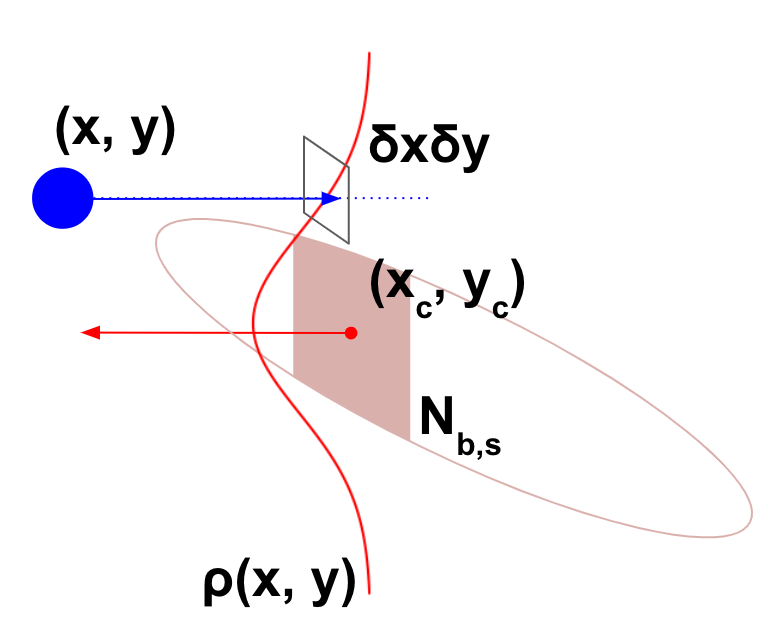
\includegraphics[width=.6\textwidth]{figures/bhabha_1.png}
	\caption{\small Schematic illustration of a single macroparticle from bunch 1 (blue) colliding with a single longitudinal slice of the opposing bunch 2 (red).  \label{fig:bhabha_1}}
\end{figure}

Figure~\ref{fig:bhabha_1} illustratres how \texttt{Xfields} computes the integrated luminosity in a collision of a single macroparticle from one beam with a single slice of the opposing beam\footnote{Note that this luminosity can be recorded in a table with the \textbf{flag\_luminosity} flag of the \texttt{BeamBeamGaussian3D} element and \textbf{lumitable} keyword in the \texttt{Xline} internal log. The recorded entries must be summed up to get the total integrated luminosity of the collision. This method has an uncertainty of $\pm10\%$ compared to the analytical formula.}. On the figure $x,y$ denote the transverse coordinates of a macroparticle in the boosted and uncoupled frame, at the collision point with a slice of the opposing bunch, corresponding to the notation $\hat{\overline{x}}^*, \hat{\overline{y}}^* $ in the previous sections. The centroid (mean) coordinate of the opposing slice, with a bunch intensity of $N_{b,s}$, is denoted by $x_c,y_c$, in the boosted, uncoupled, transported reference frame of its own bunch. \texttt{Xfields} models the charge density of a longitudinal slice as a 2D Gaussian distribution $\rho(x,y)$. Considering an infinitesimal area $\delta x \delta y$ around the transverse position $x,y$ of a given macroparticle at the collision point with the slice, one can write the number of charges with which this macroparticle will interact:

\begin{equation}
	\begin{split}
		N_e(x,y) & = N_{b,s} \rho(x,y) \delta x \delta y,
	\end{split}
	\label{eq:bhabha_1}
\end{equation}

and the integrated luminosity of the macroparticle-slice collision:

\begin{equation}
	L = \frac{N_{b,m}\cdot N_e(x,y)}{\delta x \delta y} = N_{b,m} N_{b,s} \rho(x,y),
	\label{eq:bhabha_2}
\end{equation}


where $N_{b,m}$ denotes the number of elementary charges per macroparticle.

\subsection{Virtual Photon Generation}

Equation~\eqref{eq:bhabha_2} describes the integrated luminosity of primary-primary collisions. In order to simulate the collision of the primaries with virtual photons instead, \texttt{Xfields} uses the assumption that the virtual photon distribution $N_{\gamma}(x,y)$ is proportional to that of the primary charges:

\begin{equation}
	N_{\gamma}(x,y) = nN_e(x,y),
	\label{eq:bhabha_3}
\end{equation}

where $n$ is a proportionality factor denoting the number of virtual photons corresponding to one elementary charge. The number density spectrum of virtual photons is given by:

\begin{equation}
	\frac{dn}{dxdQ^2} = \frac{\alpha}{2\pi}\frac{1 + (1 - x)^2}{x}\frac{1}{Q^2},
	\label{eq:bhabha_4}
\end{equation}

where $\displaystyle x=\frac{\hbar\omega}{E_e}=\frac{E_\gamma}{E_e}$ is the total energy of the virtual photon normalized to the primary energy and $Q^2$ is the squared virtuality of the virtual photon~\cite{Halzen:1984mc}. 

The virtual photon energies and virtualities can be drawn using the method of inverse CDF (Cumulative Distribution Function) sampling. The sampling algorithm in \texttt{Xsuite} has been adapted from \texttt{GUINEA-PIG}~\cite{guineapig}, a Particle In Cell (PIC) based single beam-beam collision simulation software. For each macroparticle in the beam, we first compute the total amount of equivalent photons using the energy of the opposite bunch slice. Subsequently, the energy and virtuality of each photon will be sampled. In the current implementation all virtual photons inherit the dynamical variables of the strong bunch slice centroid. Note that the virtual photons sampled this way will also be "macroparticles" in the sense that they represent the dynamics of all virtual photons generated by all charges in a primary macroparticle.

\subsection{Inverse Compton Scattering of Virtual Photons}

We account for the proportionality of the primary charge and virtual photon distributions described by Eq.~\eqref{eq:bhabha_3} by resampling the virtual photons for each macroparticle. With each photon, we simulate the bremsstrahlung process in the form of a set of inverse Compton scattering events. The number of Compton events can be described as:

\begin{equation}
	R = \sigma_{C,tot}(s)L = \sigma_{C,tot}(s) N_{b,m} N_{b,s} \rho(x,y),
	\label{eq:bhabha_5}
\end{equation}
where $\displaystyle s\approx\frac{4E_\gamma E_e}{m_e^2c^4}$ is the center of mass energy squared of the photon-primary Compton interaction, normalized to the rest mass of the primary~\cite{GINZBURG198347}, and $\sigma_{C,tot}(s)$ denotes the total Compton scattering cross section, given by:
\begin{equation}
	\begin{split}
		\sigma_{C,tot}(s) & = \frac{2\pi r_e^2}{s}\left[\mathrm{ln}(s+1)\left(1 - \frac{4}{s} - \frac{8}{s^2}\right).+ \frac{1}{2} + \frac{8}{s} - \frac{1}{2(s+1)^2}\right],
	\end{split}
	\label{eq:bhabha_6}
\end{equation}
with $\displaystyle r_e$ being the classical electron radius. For each event, we sample the scattered photon energy from the differential cross section:
\begin{equation}
	\begin{split}
		\frac{d\sigma_C}{dy} = \frac{2\pi r_e^2}{s}\left[ \frac{1}{1-y} + 1 - y - \frac{4y}{s(1-y)} + \frac{4y^2}{s^2(1-y)^2} \right],
	\end{split}
	\label{eq:bhabha_7}
\end{equation}
which describes the scattering of a beam of unpolarized photons on the primary charge~\cite{Schulte:331845}. Here $\displaystyle y=\frac{\hbar\omega'}{E_e}=\frac{E_\gamma'}{E_e}$ is the energy of the scattered photon in units of the total energy of the colliding primary. Given the energy $E_\gamma'$, we can compute the scattering angle of the primary and the photon as well as their momenta, using the constraints given by energy and momentum conservation. While the emitted photon spectrum corresponds to the sum of all charges represented by a macroparticle, a given macroparticle should represent the dynamics of a single primary charge. Thus, the dynamical variables of the macroparticles are updated according to energy and momentum conservation accounting for the emission of only a fraction of the photons. The latter are picked randomly based on a probability corresponding to the inverse of the number of charges per macroparticle. 

\section{Beamstrahlung}
The implementation of beamstrahlung in \texttt{Xfields} is based on \texttt{GUINEA-PIG}~\cite{guineapig}. In this section a high level summary of the modeling is presented. Further details can be found in~\cite{Yokoya:1985ab}. 

\texttt{Xfields} samples the quantum theoretical synchrotron radiation spectrum $G(v,\xi)$:

\begin{equation}
G(v,\xi) = \frac{v^2}{(1 - (1 - \xi)v^3)^2}\left( G_1(y) + \frac{\xi^2 y^2}{1 + \xi y}G_2(y) \right),
 	\label{eq:bs_1}
\end{equation}

which is normalized such that $G(v=0,\xi)=1$ and $G(v,\xi)\leq1$ for all $v$ and $\xi$. The variable $\xi$ is defined as:

\begin{equation}
	\xi=\frac{E_{crit}}{E} 
	\label{eq:bs_2}
\end{equation}

and denotes the magnitude of the quantum correction, i.e. the critical energy normalized to the energy $E$ of the primary particle in GeV undergoing the beamstrahlung process. The critical beamstrahlung energy is defined in the classical way as:

\begin{equation}
 E_{crit}=\frac{3\hbar c\gamma^3}{2\rho}
	\label{eq:bs_3}
\end{equation}

The unitless variable $y$ is related to the energy of the emitted beamstrahlung photon $E_{\gamma}$:

\begin{equation}
	y = \frac{E_{\gamma}}{E_{crit}} \frac{1}{1 - \frac{E_{\gamma}}{E}}.
	\label{eq:bs_4}
\end{equation}

Equation~\ref{eq:bs_4} can be expressed with the help of a uniform random variable $v$ as follows:

\begin{equation}
	y = \frac{v^3}{1 - v^3};~v\in U[0,1].
	\label{eq:bs_5}
\end{equation}

With these the number of beamstrahlung photons emitted in the interval [$v$, $v+\Delta v$] during a time interval $\delta_t$ can be given as:

\begin{equation}
    \Delta N_{\gamma} = p_0G(v, \xi)\Delta v,
	\label{eq:bs_6}
\end{equation}

where

\begin{equation}
p_0 = \frac{2^{\frac{2}{3}}}{\Gamma(\frac{4}{3})} \frac{\alpha\gamma\delta_t}{\rho}\approx 25.4\cdot \frac{E \delta_t}{\rho}
	\label{eq:bs_7}
\end{equation}

is a scaling factor dependent on the relativistic $\gamma$ of the primary, the instantaneous bending radius $\rho$ and the fine structure constant $\alpha$. The bending radius of each macroparticle in the electromagnetic field of a given longitudinal slice of the opposite bunch is obtained from the radial kick:

\begin{equation}
	F_r^*=r_{pp}\sqrt{F_x^{*2} + F_y^{*2}},
	\label{eq:bs_8}
\end{equation}
\begin{equation}
	\rho=\frac{1}{F_r^*},
	\label{eq:bs_9}
\end{equation}

with $r_{pp}=\frac{1}{1 + \delta}=\frac{p}{p_0}$. In the \texttt{Xfields} \texttt{BeamBeamGaussian3D} element the time interval $\delta_t$ is expressed as a longitudinal distance $\Delta z$, which is the distance the macroparticle travels between two consecutive longitudinal slices and it corresponds to the bin width of the longitudinal slicing.

Figure~\ref{fig:bs_1} shows the beamstrahlung photon number density $p_0G(v,\xi)$ for a fixed value of $p_0$ and $\xi$. The area in the region C is the mean number of beamstrahlung photons emitted during an interval $\delta_t$, i.e. a passage through one longitudinal slice of width $\Delta z$.

\begin{figure}[h]
	\centering
	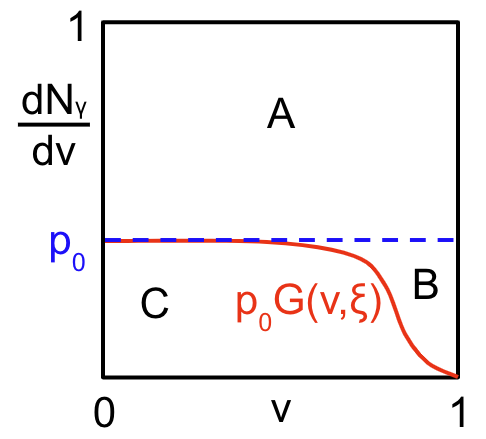
\includegraphics[width=.5\textwidth]{figures/bs_1.png}
	\caption{\small Schematic illustration of the number density function of beamstrahlung photons $p_0G(v,\xi)$ (red curve) for a given $p_0$ (blue dashed line) and $\xi$, as a function of $v$.  \label{fig:bs_1}}
\end{figure}

The functions $G_1(y)$ and $G_2(y)$ are defined as follows:

\begin{equation}
	\begin{split}
		G_1(y) & = \frac{\sqrt{3}\Gamma(\frac{1}{3})}{2^{\frac{5}{3}}\pi} \int\limits_{y}^{\infty} K_{\frac{5}{3}}(x) dx, \\
		G_2(y) & = \frac{\sqrt{3}\Gamma(\frac{1}{3})}{2^{\frac{5}{3}}\pi}  K_{\frac{2}{3}}(y).
	\end{split}
 	\label{eq:bs_10}
\end{equation}

Equations~\ref{eq:bs_10} are evaluated numerically with the below approximate formulas:

\begin{equation}
	\begin{split}
	0 \leq y \leq 1.54 & \\
	G_1(y) & = y^{-\frac{2}{3}} (1 - 0.8432885317\cdot y^{\frac{2}{3}} + 0.1835132767\cdot y^2 \\
	& - 0.0527949659\cdot y^{\frac{10}{3}} + 0.0156489316\cdot y^4) \\
	G_2(y) & = y^{-\frac{2}{3}} (0.4999456517 - 0.5853467515\cdot y^{\frac{4}{3}} \\
	& + 0.3657833336\cdot y^2 - 0.0695055284\cdot y^{\frac{10}{3}} + 0.0191803860\cdot y^4) 	\end{split}
\label{eq:bs_11}
\end{equation}
\begin{equation}
	\begin{split}
	1.54 < y \leq 4.48 & \\	
	G_1(y) & = \frac{2.066603927 - 0.5718025331\cdot y + 0.04243170587\cdot y^2}{-0.9691386396 + 5.651947051\cdot y - 0.6903991322\cdot y^2 + y^3} \\
	G_2(y) & = \frac{1.8852203645 - 0.5176616313\cdot y + 0.03812218492\cdot y^2}{-0.4915880600 + 6.1800441958\cdot y - 0.6524469236\cdot y^2 + y^3}
	\end{split}
\label{eq:bs_12}
\end{equation}

\begin{equation}
\begin{split}
	4.48 < y \leq 165.0 & \\	
	G_1(y) & = 	\frac{e^{-y}}{\sqrt{y}}\cdot \frac{1.0174394594 + 0.5831679349\cdot y}{0.9949036186 + y} \\
	G_2(y) & = \frac{e^{-y}}{\sqrt{y}}\cdot \frac{0.2847316689 + 0.5830684600\cdot y}{0.3915531539 + y}.
	\end{split}
 	\label{eq:bs_13}
\end{equation}

For $y>165$ the model assumes no radiation. With these one can simulate beamstrahlung emission by first drawing a random uniform number $p$. The condition $p>p_0$ corresponds to region A on Fig.~\ref{fig:bs_1}, therefore no photons are emitted. In the other case a second random uniform number $v$ is drawn, and Eq.~\ref{eq:bs_1} is computed. If $p<p_0G(v,\xi)$ is satisfied (region C) a photon is emitted with an energy

\begin{equation}
\frac{E_\gamma}{E} = \frac{\xi v^3}{1 - (1 - \xi)v^3},
	\label{eq:bs_14}
\end{equation}

otherwise no photon is emitted (region B). The generated beamstrahlung photons are themselves macroparticles in the sense that they represent the dynamics of all photons generated by all charges in a primary macroparticle.
\newpage

\section*{Appendices}
\addcontentsline{toc}{section}{Appendices}


\begin{appendices}
\renewcommand{\thesubsection}{A\arabic{subsection}}



\subsection{Detailed explanation of "the boost" transformation}
\label{app:boost}
The reference frame transformation used in Sec.~\ref{sec:directboost} can be written as \cite{hirata, beam_beam}:
\begin{equation}
\left( \begin{matrix}
\sigma^*\\
x^*\\
s^*\\
y^*
\end{matrix} \right) = A^{-1}{R_{\mathrm{CP}}}^{-1}L_{\mathrm{boost}}R_{\mathrm{CA}}R_{\mathrm{CP}}A
\left( \begin{matrix}
\sigma\\
x\\
s\\
y
\end{matrix} \right) 
\end{equation}

Here $A$ is the matrix transforming the accelerator coordinates (Courant-Snyder) to Cartesian coordinates:

\begin{equation}
\left( \begin{matrix}
ct\\
X\\
Z\\
Y
\end{matrix} \right) = A
\left( \begin{matrix}
\sigma\\
x\\
s\\
y
\end{matrix} \right) =
\left( \begin{matrix}
-1 &0 &1&0\\
0 &1 &0&0\\
0 &0 &1&0\\
0 &0 &0&1
\end{matrix} \right) 
\left( \begin{matrix}
\sigma\\
x\\
s\\
y
\end{matrix} \right)
\end{equation}

$R_{\mathrm{CP}}$ is a rotation matrix bringing the crossing plane to the $X-Z$ plane:
\begin{equation}
R_{\mathrm{CP}}=
\left( \begin{matrix}
1 &0 &1&0\\
0 &\cos\alpha &0&\sin\alpha\\
0 &0 &1&0\\
0 &-\sin\alpha &0&\cos\alpha
\end{matrix} \right) 
\end{equation}

$R_{\mathrm{CA}}$ is a rotation matrix moving to the barycentric reference frame (in which the two beams are symmetric with respect to the s-axis):
\begin{equation}
R_{\mathrm{CA}}=
\left( \begin{matrix}
1 &0 &0&0\\
0 &\cos\phi&\sin\phi &0\\
0 &-\sin\phi&\cos\phi &0\\
0 &0 &0&1
\end{matrix} \right) 
\end{equation}

$L_{\mathrm{boost}}$ is the matrix defining a Lorentz boost in the direction of the rotated X-axis:
\begin{equation}
L_{\mathrm{boost}}=
\left( \begin{matrix}
1/\cos\phi &-\tan\phi &0&0\\
-\tan\phi &1/\cos\phi&0 &0\\
0 &0&1 &0\\
0 &0 &0&1
\end{matrix} \right) 
\end{equation}

The momenta are transformed similarly \cite{beam_beam}:

\begin{equation}
\left( \begin{matrix}
\delta^*\\
p_x^*\\
h^*\\
p_y^*
\end{matrix} \right) = 
B^{-1}{R_{\mathrm{CP}}}^{-1}L_{\mathrm{boost}}R_{\mathrm{CA}}R_{\mathrm{CP}}B
\left( \begin{matrix}
\delta\\
p_x\\
h\\
p_y
\end{matrix} \right) 
\end{equation}

where the transformation from accelerator to Cartesian coordinates given by:

\begin{equation}
\left( \begin{matrix}
E/c-p_0\\
P_x\\
P_z-p_0\\
P_y
\end{matrix} \right) = p_0
\left( \begin{matrix}
1 &0 &0&0\\
0 &1&0 &0\\
0 &0&-1 &0\\
0 &0 &0&1
\end{matrix} \right)
\left( \begin{matrix}
\delta\\
p_x\\
h\\
p_y
\end{matrix} \right) 
\end{equation}

As explaned in Sec.\ref{sec:directboost} not all particles with $s=0$ are fixed points of the transformation, therefore a drift  back to s=0 needs to be performed as we are tracking w.r.t. $s$ and not w.r.t. time. The net effect of the transformation is to move from the reference frame of the weak beam to the boosted barycentric frame.

%\section{Some equations for slides}
%
%\begin{equation}
%\sin \theta = 0
%\end{equation}

\subsection{Constant charge slicing}
\label{app:slicing}
We consider a Gaussian longitudinal bunch distribution:

\begin{equation}
\lambda(z) = \frac{1}{\sigma_z \sqrt{2\pi}}e^{-\frac{z^2}{2\sigma_z^2}} 
\end{equation}

We introduce the cumulative distribution function:

\begin{equation}
Q(z) = \int_{-\infty}^{z} \lambda(z')dz' = \frac{1}{2}+\frac{1}{2}\mathrm{erf}\left(\frac{z}{\sqrt{2}\sigma_z}\right)
\label{cumul}
\end{equation}

We define longitudinal cuts $z^{\mathrm{cut}}_n$ such that the bunch is sliced in $N$ sections having the same charge:

\begin{equation}
Q(z^{\mathrm{cut}}_n) = \frac{n}{N}
\label{constsli}
\end{equation}

Replacing \ref{constsli} in \ref{cumul} we obtain:

\begin{equation}
z^{\mathrm{cut}}_n = \sqrt{2} \sigma_z \mathrm{erf}^{-1}\left( \frac{2n}{N}-1\right)
\end{equation}

For each slice we need to find the longitudinal centroid position. For generic slice having edges $z_1$ and $z_2$ the centroid position can be written as:

\begin{equation}
z^{centroid}= \frac{1}{Q(z_2) - Q(z_1)}\int_{z_1}^{z_2} z \lambda(z)dz = \frac{\sigma_z}{\sqrt{2\pi}\left(Q(z_2) - Q(z_1)\right)}\left(e^{-\frac{z_1^2}{2\sigma_z^2}}-e^{-\frac{z_2^2}{2\sigma_z^2}}\right)
\end{equation}

\subsection{Considerations on the $\Sigma$-matrix description}
\label{app:sigma}

Given the reduced $\Sigma$-matrix of the beam (including only position terms, no momenta):
\begin{equation}
\Sigma = \left(
\begin{matrix}
{\Sigma}_{11} & {\Sigma}_{13}\\
{\Sigma}_{13} & {\Sigma}_{33}
\end{matrix}
\right)
\end{equation}



 the distribution for a Gaussian beam can be written as:
\begin{equation}
\rho(\textbf{x}) = \rho_0 e^{-\textbf{x}^{\mathrm{T}} \Sigma^{-1}\textbf{x}}
\end{equation}

Points having same density lie con ellipses defined by the equation:
\begin{equation}
\textbf{x}^\mathrm{T}\Sigma^{-1}\textbf{x} = \mathrm{const.}
\label{eqellipse2}
\end{equation}

As $\Sigma$ is symmetric, it can be diagonalized:
\begin{equation}
\Sigma = \textbf{V} \textbf{W} \textbf{V}^{T}
\label{diagsigma}
\end{equation}

where the matrix $\textbf{V}$ has in its columns the eigenvectors of $\Sigma$ and $\textbf{W}$ is a diagonal matrix with the corresponding eigenvalues:
\begin{equation}
W = \left(
\begin{matrix}
\hat{\Sigma}_{11} & 0\\
0 & \hat{\Sigma}_{33}
\end{matrix}
\right)
\end{equation}

 $\textbf{V}$ is a unitary matrix (eigenvectors are ortho-normal):
\begin{equation}
\textbf{V} \textbf{V}^{T} = \textbf{I} \Rightarrow \textbf{V}^{-1} = \textbf{V}^{T}
\label{unitarity}
\end{equation}

\textbf{V} can be used to transform coordinates from the initial frame to the de-coupled frame:

where $\hat{\textbf{x}}$ are the coordinates in the decoupled frame, i.e. the projections of of $\textbf{x}$ on the eigenvectors:
\begin{equation}
\hat{\textbf{x}}= \textbf{V}^{T}\textbf{x}
\label{vartransform}
\end{equation}

Combining Eqs.~\ref{diagsigma} and~\ref{unitarity} we can write:

\begin{equation}
\Sigma^{-1} = \textbf{V} \textbf{W}^{-1} \textbf{V}^{T}
\end{equation}

This can be replaced in Eq.~\ref{eqellipse2}, re-writing the equation of the ellipse as:
\begin{equation}
\textbf{x}^\mathrm{T}\textbf{V} \textbf{W}^{-1} \textbf{V}^{T}\textbf{x} = \mathrm{const.}
\end{equation}

Using Eq.~\ref{vartransform} we obtain the equation of the ellipse in the reference system of the eigenvectors:
\begin{equation}
\hat{\textbf{x}}^\mathrm{T}\textbf{W}^{-1} \hat{\textbf{x}} = \mathrm{const.}
\end{equation}
which can be rewritten in the familiar form:
\begin{equation}
\frac{\hat{x}^2}{\hat{\Sigma}_{11}}+\frac{\hat{y}^2}{\hat{\Sigma}_{33}}=\mathrm{const.}
\end{equation}

Once the $\Sigma$-matrix is assigned, the one-sigma ellipse can be drawn by the following procedure:
\begin{itemize}
\item We diagonalize $\Sigma$ and we generate an auxiliary matrix defined as:
\begin{equation}
\textbf{A} = \textbf{V} \sqrt{\textbf{W}} \textbf{V}^{T}
\end{equation}
\item We generate a set of points in the unitary circle
\begin{equation}
\textbf{z} = \left[
\begin{matrix}
\cos t\\
\sin t
\end{matrix}
\right]
\end{equation}
\item We apply $ \textbf{A} $ to t to generate points on the one-sigma ellipse:
\begin{equation}
\textbf{x}_{1\sigma} = \textbf{A} \textbf{z}
\end{equation}
\end{itemize}

This can be verified as follows:
\begin{align}
{\textbf{x}_{1\sigma}}^\mathrm{T}\Sigma^{-1}\textbf{x}_{1\sigma} 
&= \textbf{z}^\mathrm{T}\textbf{A}^\mathrm{T}\Sigma^{-1}\textbf{A}\textbf{z} = \textbf{z}^\mathrm{T}(\textbf{V} \sqrt{\textbf{W}} \textbf{V})(\textbf{V}^{T} \textbf{W}^{-1} \textbf{V}^{T})(\textbf{V}\sqrt{\textbf{W}} \textbf{V}^{T}) \textbf{z} \nonumber
\\&=\textbf{z}^\mathrm{T}\textbf{V} \sqrt{\textbf{W}}  \textbf{W}^{-1} \sqrt{\textbf{W}} \textbf{V}^{T}\textbf{z}
= \textbf{z}^\mathrm{T}\textbf{V}  \textbf{V}^{T}\textbf{z} 
= \textbf{z}^\mathrm{T}\textbf{z} = 1
\end{align}

\end{appendices}
